\chapter{Data Acquisition}

\section{Background}
\subsection{HTML and Xpath}

Internet webpages are written in a markup language called HTML, (HyperText Markup Language). When a webpage is accessed, the html code is sent over the internet to the user, and the browser e.g. Firefox, interprets it and displays the webpage in a human readable format. 

A program written to automatically interpret webpages and extract information, is known as a `scraping' program. The program must process the raw HTML file and access the useful information on the page in an automated fashion. Information is arranged in an html document in a tree-like structure, see Figure \ref{fig:HTMLTREE}. This example page would display in a browser as a table with 3 rows, each row containing `Table Data A/B/C'. The method of tree traversal is by specifying a path through the document tree on the right, using an `xpath'. 
\begin{figure}[H]
    \centering
    \textbf{HTML and XPaths}\par\medskip
    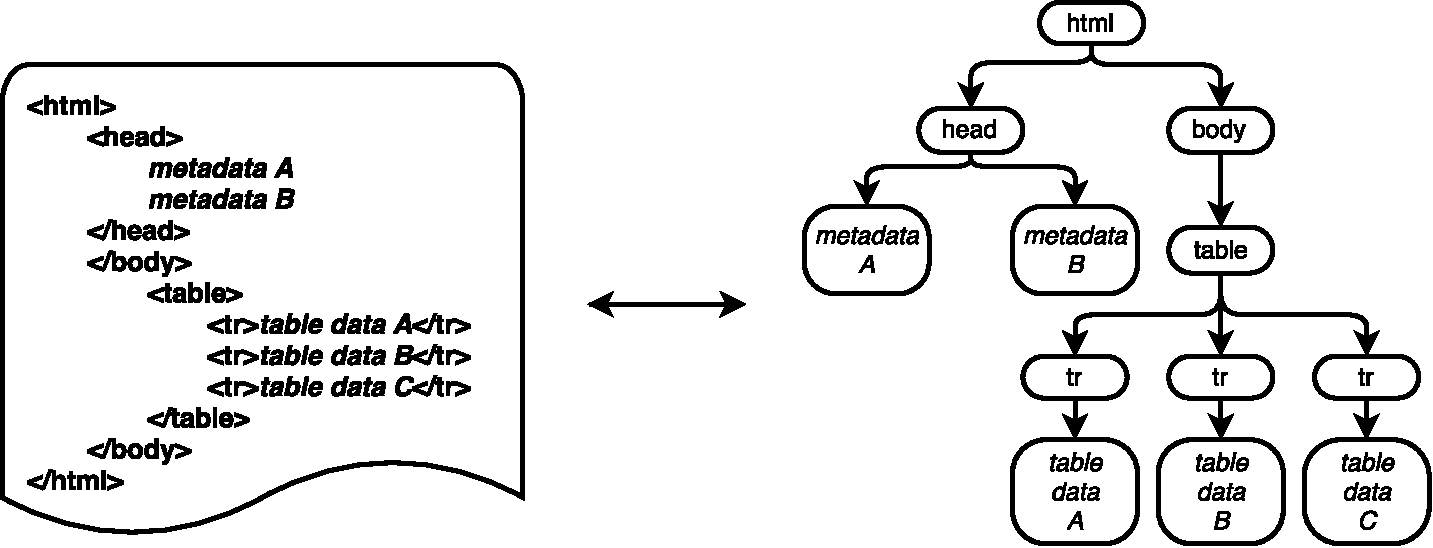
\includegraphics[scale=0.7]{Data_Acquisition/html_tree.pdf}
    \caption{Tree representation of HTML code. The html code here displays a table with 3 rows. The page has two peices of metadata associated with it, stored in the `head'.\label{fig:HTMLTREE}}
\end{figure}
Xpaths are just directions to take down the document tree to access the desired information. In order the `scrape' the data in the table, the following xpath could be used:
\begin{center}
\texttt{//html/body/tr/*}
\end{center}
In order to scrape information on a page, the xpath must be known. 
This presents an immediate problem, as scraping a millions of webpages requires millions of potentially different xpaths to be known. It is clearly impractical to specify them manually. Two possible solutions were attempted.
The challenge of large scale scraping is how to identify useful data on the page and collect it, without manually specifying very many xpaths.
\section{Automatic Xpath Generation}
The initial approach was to attempt to analyse the html tree to automatically recognise where useful tabulated or listed data was. The program started at the root of the tree and repeatedly followed the branch with the most `repeated structure'. The recursive algorithm is summarised below:
\begin{sloppypar}
\begin{enumerate}
\item \texttt{Count \# of descendents of each child node}
\item \begin{enumerate}
\item \texttt{Calculate the pairwise similarities between all child nodes}
\item \texttt{Consider  two nodes similar if pairwise similarity is above a heuristic threshold}
\item \texttt{Calculate proportion of nodes that are considered similar}
\end{enumerate}
\item \texttt{If proportion calculated in (c) is above a heuristic threshold, this node represents a store of information, and the xpath has been found. Otherwise, move to child node with highest \# of descendants, return to step (1)}
\end{enumerate}
\end{sloppypar}
The heuristic thresholds are adjustable parameters. The approach was successful for webpages with large numbers of records, laid out in repeating fashion, but performs poorly for smaller tables or lists of data. As such it was not flexible enough for the task of scraping large for chemical data, and was not implemented in final solution.
\section{Collection Strategy}
The goal set was to build a database of chemical information freely available on the internet. This section describes how this task was addressed.
As generating xpaths proved unsuitable, a new strategy was required. Chemical information is often disseminated as published articles. Modern papers are accompanied by a DOI. By programmatically collecting DOIs, (see section \ref{sec:DOI}) it is possible to build up a large database of chemical information (see section \ref{sec:SCRAPINGPROGRAM})
\subsection{Document Object Identifiers}
\label{sec:DOI}
DOIs (document object identifiers) are digital labels for journal articles. DOIs are issued by a number of accredited bodies, with the vast majority of chemistry related articles issued by Crossref.\footnote{Crossref is a not-for-profit body comprised from Publishers International Linking Association (PILA), an association of many academic publishers} \cite{CROSSREF-FORMATION}. By pre-pending a DOI string with the url stub \texttt{http://dx.doi.org/}, the International DOI foundation (IDF) service will redirect the request to the publisher's website to display the article the DOI refers to. The structure of a DOI is shown in Figure \ref{fig:DOI}.
\begin{figure}[H]
    \centering
    \textbf{Anatomy of a DOI}\par\medskip
    \includegraphics[scale=0.15]{Data_Acquisition/DOI2.png}
    \caption{Doi structure. The structure consists of a numeric prefix (X and Y must be integers) and alphanumeric suffix (Z can be any Unicode encoded character) \label{fig:DOI}}
\end{figure}
DOIs consist of a prefix and suffix. The prefix is subdivided into the ‘Directory Indicator’ (always integer ‘10’) separated from the ‘Registrant Code’, assigned by the issuing body. Registrant codes are numeric and can be a minimum of 3 integers. Registrant codes can have further subdivisions separated by full stops. The suffix is provided by the registrant themselves. It can take any form as long as it is encodable by UTF-8.


It was possible to write a `Regular Expression pattern' matcher (regex) to automatically recognise DOIs within a body of text due to this defined structure.\ref{fig:REGEX} The flexibility of the registrant code specification means that DOIs cannot always be unambiguously identified in html documents. 
\begin{figure}[H]
    \centering
    \textbf{Pattern Matching Procedure for DOIs}\par\medskip
    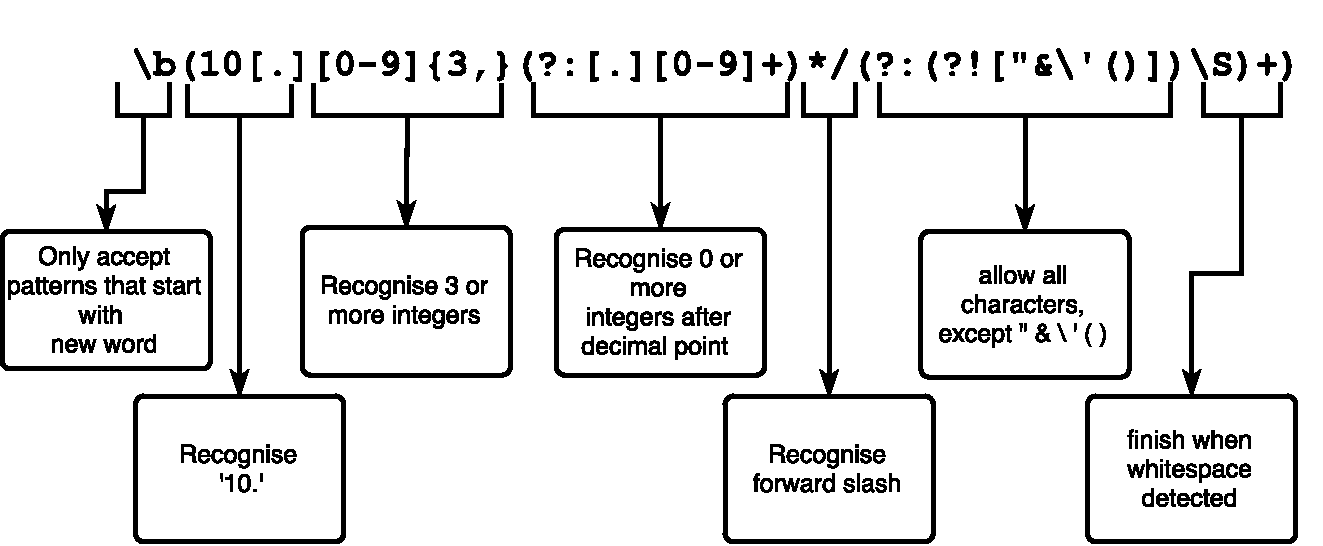
\includegraphics[scale=0.5]{Data_Acquisition/Regex.pdf}
    \caption{Perl Syntax Code that can identify the vast majority of DOIs within free text) \label{fig:REGEX}}
\end{figure}
Despite this, the regex is sufficient to identify 90.4\% of the dois on the Cambridge University Chemistry Department website \url{http://www.ch.cam.ac.uk/publications}. 
\subsection{Scraping Program}
\label{sec:SCRAPING_PROGRAM}
The Regex approach does not require any xpath in order to extract dois from a webpage. This facilitates large scale scraping from a large set of websites.
The meta-data associated with a DOI can be accessed using an online API exposed by Crossref.Further metadata can be accessed by following the \texttt{http://dx.doi.org/\{DOI\}} redirecting service by DOI\circledR .org. to visit publishers's websites to collect any remaining metadata. 


The scaping program was thus written in python to collect DOIs from a list of webpages and collect metadata in a 2 stage process. The Crossref API provides article titles, journals,authors, publisher and publication date meta-data, but not article abstracts. These had to be collected by visiting publisher webpages, and collecting with hand written xpaths. \footnote{Since there are not a great many different publisher websites, only 26 publisher xpaths were required for decent capture coverage.} The procedure is summarised in figure \ref{fig:Cherry} below:
\begin{figure}[H]
    \centering
    \textbf{Scraping Procedure}\par\medskip
    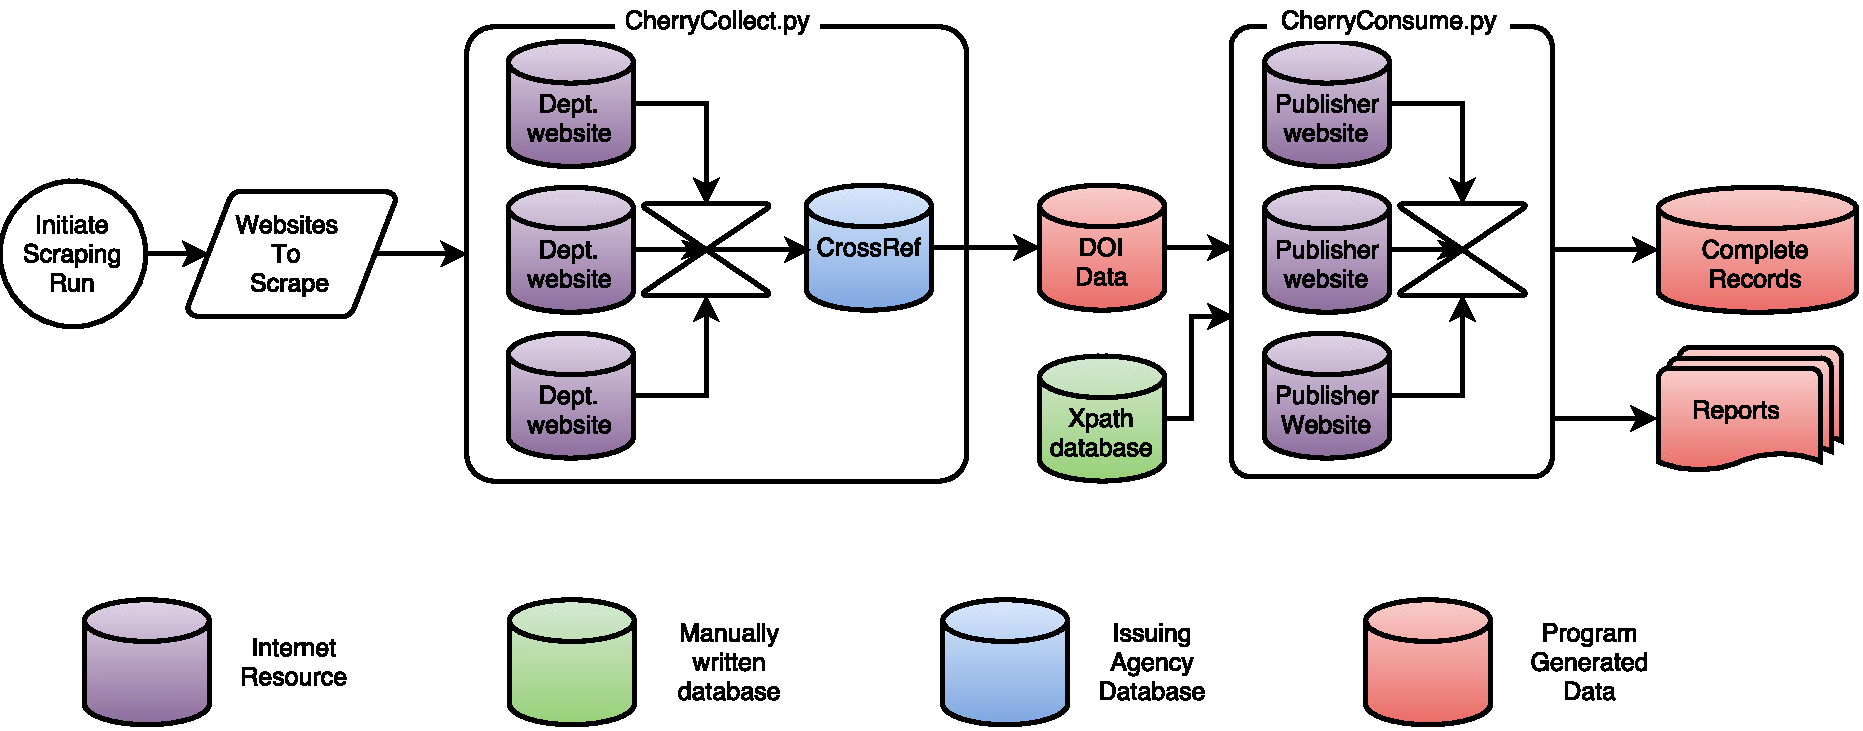
\includegraphics[scale=0.5]{Data_Acquisition/Cherry.pdf}
    \caption{The data flow of the scraping program. An inputted list of websites to scrape are visited and dois are extracted in the process described in \ref{sec:DOI}. The Crossref API service is then used to verify the extracted dois, and collects available meta-data. The program then accesses publisher webpages and collects the abstracts. The program also produces explanation of capture failures and some general statistics}
     \label{fig:Cherry}
\end{figure}
The programmatic steps depicted in \ref{fig:Cherry} are:
\begin{sloppypar}
\begin{enumerate}
\item \texttt{Request the webpage from the inputted list}
\item \texttt{Process the htlm and extract dois}
\item \texttt{Using the Crossref Online API, verify the extracted DOIs exist.}
\item \texttt{Crossref yields metadata:}
\begin{itemize}
\item \texttt{Title}
\item \texttt{Journal}
\item \texttt{Publisher}
\item \texttt{Authors}
\item \texttt{Publication Date}
\end{itemize}
\item \texttt{for each doi, follow the doi using \texttt{http://dx.doi.org/\{DOI\}}}
\item \texttt{use xpath to collect article abstracts.}
\end{enumerate}
\end{sloppypar}
The program exports complete records as .json files, but is also able to feed directly to a MongoDB database instance. Obtaining an input list of websites to scrape was the next area of focus which is described in sections \ref{sec:UKSCRAPE} and \ref{ sec:CROSSREFSCRAPE} 
\section{Collection Results}
\subsection{UK University Department scraping}
\label{sec:UKSCRAPE}
The program was first used to collect the data from the UK. The Goodman group's website hosts a list of UK chemistry departments \url{http://www-jmg.ch.cam.ac.uk/data/c2k/uk.html}. The list was manually checked and some urls were changed for efficiency of landing targets to give a list of 68 departments\footnote{Details can be found in the appendix}. The program was set to collect dois on all the pages it could find at these websites and collect metadata in the described in section\ref{sec:SCRAPING_PROGRAM}.
This resulted in a collection of:
\begin{table}[h!]
\label{tab:UKSCRAPERES}
\caption{UK Scraping results}
\begin{center}
\begin{tabular}{||l|l|l||}
\hline
Process & \# records & \% of maximum yield\\
\hline
Dois collected & 22442 & 100.0\%\\
Dois found with metadata & 22397 & 99.8\%\\
Articles successfully resolved & 16363 & 72.9\%\\
Losses due to failed requests & 2753 & 12.3\%\\
Program errors & 133 & 0.6\%\\
Missing Publication Errors & 3148 & 14.0\% \\
\hline
\end{tabular}
\end{center}
\end{table}
Conversion losses were due to 4 components. 45 losses were due to non-existant dois. 2753 losses were due to request errors such as could be due to 404 : not-found errors or permission problems. 
133 conversion losses were due to the program throwing internal errors.
3148 conversions were lost due missing publication xpaths. The 26 specified xpaths were sufficient to convert 83.8\% of successful requests. This was deemed acceptable, as most major publishers had been covered \footnote{see appendix for list of covered publishers}, and the missing publishers each covered a small number of articles it would take another 11 xpaths of the missing most popular publishers to increase the conversion rate from 83.8\% to 90\%.
The efficiency is depicted in \ref{fig:UKSANK}

\begin{figure}[H]
    \centering
    \textbf{Efficiency of UK Department Scraping}\par\medskip
    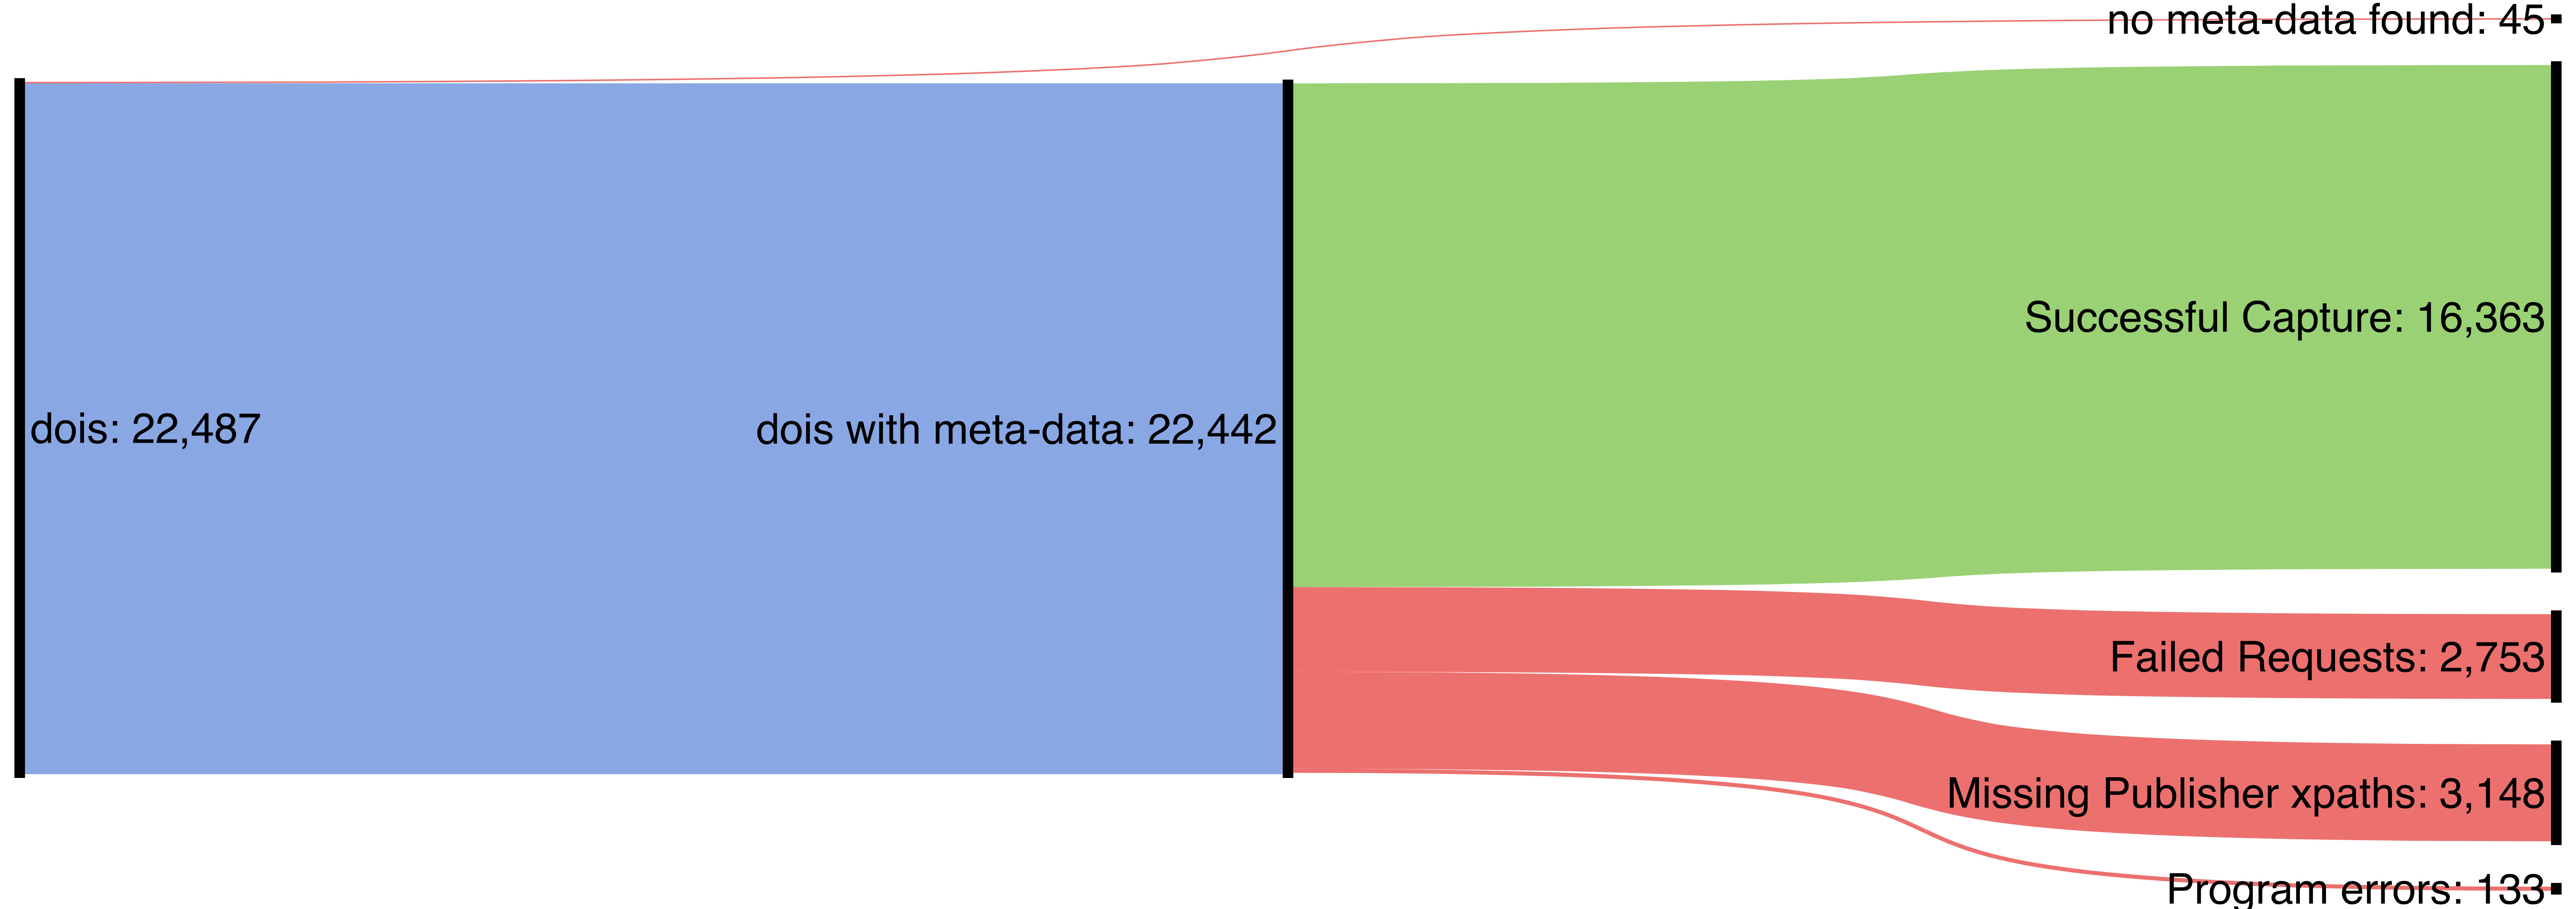
\includegraphics[scale=0.07]{Data_Acquisition/uk_sankey.png}
    \caption{The loss processes are coloured red, successfully captured full records in green, and the maximum possible yield in blue.}
     \label{fig:UKSANK}
\end{figure}

Interestingly, 9467 out of 16363 successful collections were sourced from \url{http://www.ch.cam.ac.uk}. This could be because the Cambridge Chemistry department has its own website domain name where most of its data is hosted, whereas other departments` data is hosted on central university domain names. The scraping program was confined to scrape only webpages belonging directly to chemistry department websites, not the university website as a whole. As a result, it is worth baring in mind that the Cambridge chemistry department may be overrepresented in the UK chemistry data set.

\subsection{Very Large Scale Scraping}
\label{sec:CROSSREFSCRAPE}
The collection procedure above was successful. However, in order for the machine learning analysis on the collected meta-data to be successful, much more training data was required. To this end, it was necessary to collect many more records. One approach would have been expand the scrape to world-wide chemistry departments, and other learn\`{e}d bodies. However, Crossref also exposes a search service that can be used to query it's vast internal database. The program was then set up to query the Crossref service for search terms `Chemistry', `Chemical', 'Molecule' and 'Molecular' for journal articles and journal titles. This suggested possible yields in the millions of articles. 

The program was thus set up to scrape the search results pages of these queries. Because the scraping job was so large, the program was instructed to run the scrape in two distinct sessions. Firstly, it was to collect DOIs and get easily avaiable metadata. The results of this scrape were to be examined before setting off the second stage, collecting abstracts from publisher web pages. 

After the doi and-meta data scraping run, the program had collected 1,267,495 records, which was deemed very successful, and would provide enough data to train a powerful machine learning algorithm.

The records were then inspected and publisher distributions were considered. Some of this analysis is presented in \ref{sec:SCRAPEANALYSIS}. After careful considerations of request server loads and predicting capture probabilities, the second half of the scraping routine was set off to run for 3 days.
\label{sec:CROSSREFSCRAPE}
\subsection{Problems with ACS and Taylor and Francis}
Some publishers automatically track number of requests sent to their site as they wish to discourage automatic scraping of their data. Scraping their websites is not illegal, and the data collected was freely available, not behind paywalls, or protected. However, during the scraping run, a bug in the randomisation of request frequencies resulted in the scraping being detected by publishers ACS (American Chemical Society) and Taylor and Francis. Both publishers responded by banning the IP address of the computer running the program. The department Librarians were able to restore access, and it was agreed that no further large scale scraping runs would be performed. 

Taylor and Francis banned the IP address after it detected over 100 requests were made within 5 minutes. This corresponds to a request every 3 seconds. This is modest server load compared to other publishers, and was not predicted to cause problems.

The ACS banning occurred because of a nuanced bug in the randomisation of requests. The program was instructed to take a random publisher's doi per request. However, since the largest publisher of chemistry articles was ACS, the program eventually the other publishers papers, until it had only ACS papers to `randomly' draw requests from. This meant the request frequency to the ACS server went up dramatically. This uptick broke the threshold of allowed requests at the ACS server which then banned the IP (approximately 10 requests a second).

\begin{figure}[H]
    \centering
    \textbf{ACS BANNING}\par\medskip
    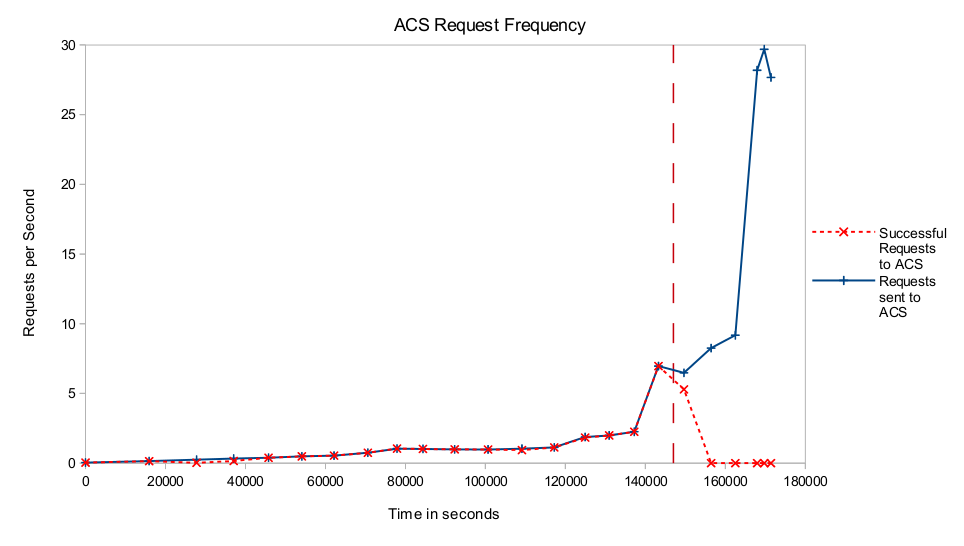
\includegraphics[scale=0.8]{Data_Acquisition/ACS_crash_line.png}
    \caption{The request frequency is plotted in blue, the received pages frequency in red. The vertical dashed line shows where the server detected the scape and banned the IP.}
     \label{fig:ACSBAN}
\end{figure}
The program was capable of making a total number of approximately 30 requests per seconds.As can be seen in figure \ref{fig:ACSBAN}, the program began to run out of requests to other publishers after approximately 140,000 seconds, resulting in an increase in  the proportion of total requests per second going to ACS. The banning occurred after approximately 150,000 results, after which there were no more responses to requests.
\subsection{Analysis of Collected data}
The yield of the large scale scraping run was cut significantly by the ACS banning event. A summary is tablulated in \ref{sec:LARGESCRAPERES}
\begin{table}[h!]
\label{tab:LARGESCRAPERES}
\caption{Large Scale Scraping Results}
\begin{center}
\begin{tabular}{||l|l|l||}
\hline
Process & \# records & \% of maximum yield\\
\hline
DOIS collected in stage 1 &  1267495 &100.0\%\\
\hline
Predicted maximum capture & 1071506 &  84.5\%\\
Predicted Capture without ACS & 581797 & 45.9\%\\
\hline
Articles successfully captured & 714370 & 56.4\%\\
Losses to failed requests (excluding ACS)& 53743 & 4.2\%\\
Losses to ACS banning & 303393 & 23.9\%\\
Missing Publications \& Program Errors & 195989 & 15.5\%\\
\hline
\end{tabular}
\end{center}
\end{table}
The overall efficiency of the process is 56.4\%. This is mainly down to ACS ban reducing the number of successfully collected articles. Excluding the ACS lost records, the program's efficiency jumps to 74.0\%, similar to the efficiency of the UK scraping run (section \ref{sec:UKSCRAPE}).  The efficiency is shown graphically in \ref{fig:LARGESANK}
\begin{figure}[H]
    \centering
    \textbf{Efficiency of Large Scale Scraping}\par\medskip
    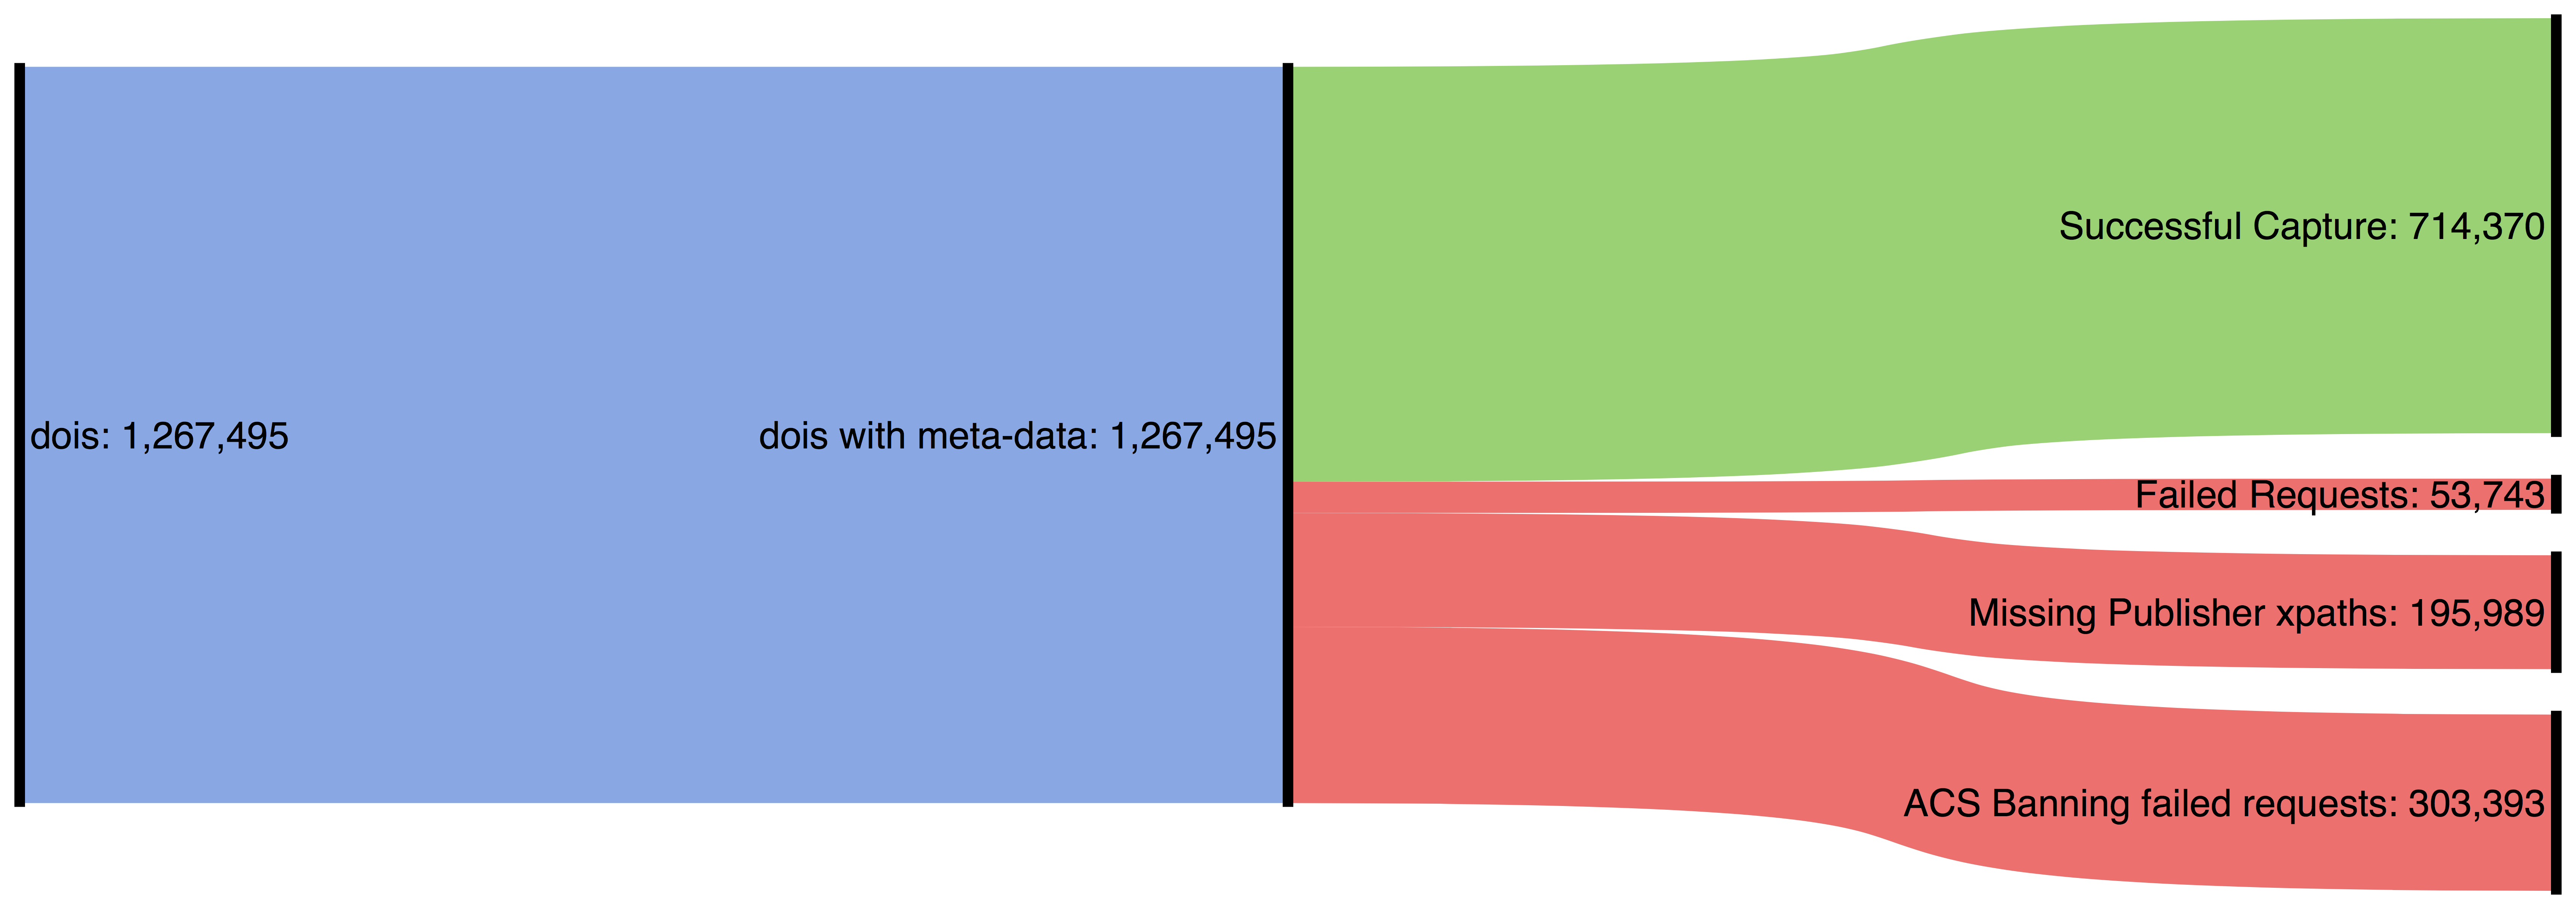
\includegraphics[scale=0.07]{Data_Acquisition/large_sankey.png}
    \caption{The loss processes are coloured red, successfully captured full records in green, and the maximum possible yield in blue.}
     \label{fig:LARGESANK}
\end{figure}

The successfully captured 714,370 records were then inspected and merged with the UK results. Records were then rejected with short titles or short abstracts (likely to be addenda, informal articles, retractions etc.) Records were also removed if the majority of the title and abstract were not written in acscii characters \footnote{ascii is an encoding for English characters a-z, A-Z, some punctuation and 1-9.} (removing majority Japanese and Chinese script). This was done to provide better quality data for training the algorithm described in chapter \ref{chapt:ALGORITHM}. This filtering resulted in a final database of 464712 articles. The entire database formation process is shown in figure \ref{fig:DATABASES}.
\begin{figure}[H]
    \centering
    \textbf{Summary of Data Preparation}\par\medskip
    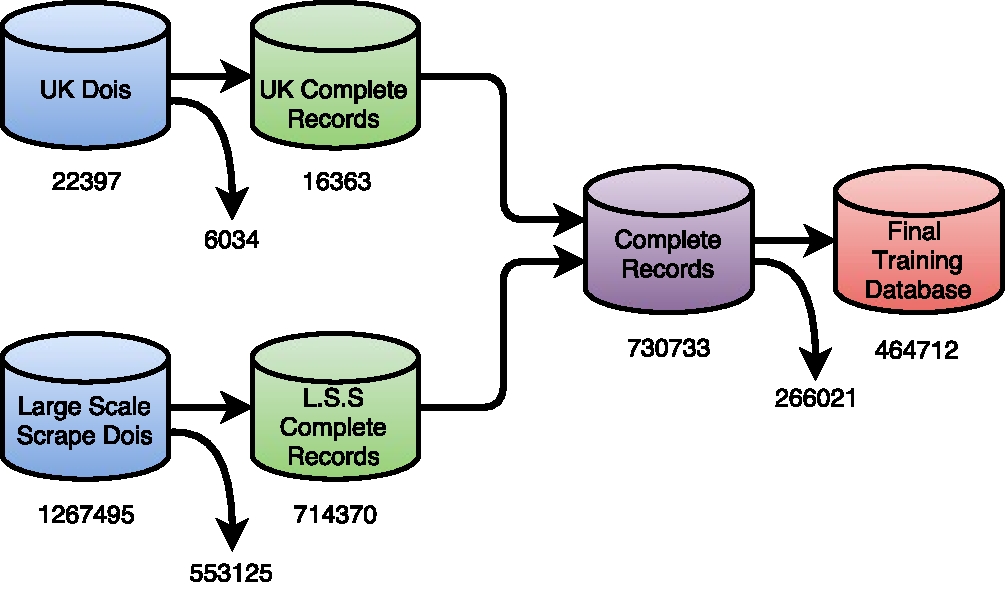
\includegraphics[scale=0.6]{Data_Acquisition/Databases.pdf}
    \caption{Blue databases represent data with dois and metadata. Green databases represent meta-data, dois and abstracts. The purple database is the combined complete records, and the red database is the data deemed suitable for the training algorithm. database sizes and losses are annotated.}
     \label{fig:DATABASES}
\end{figure}


It was instructive to examine these databases and derive some simple statistical results. The following section briefly explores some of these.
\subsubsection{Observations}
The publisher `market share' can be approximated from examining the Large Scale Scape Doi database, shown in \ref{fig:PUBPI}. 
\begin{figure}[H]
    \centering
    \textbf{Publisher Share in Chemistry Literature}\par\medskip
    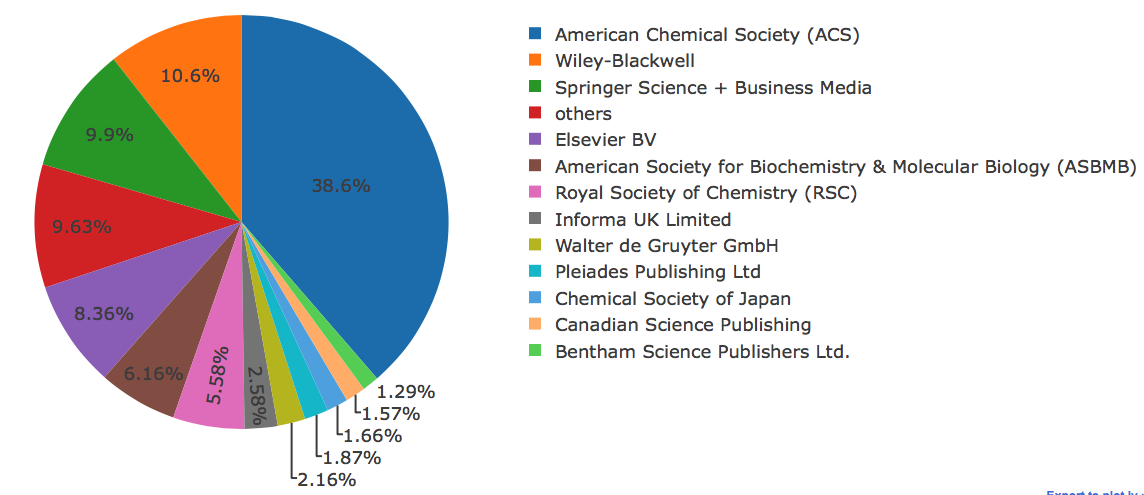
\includegraphics[scale=0.4]{Data_Acquisition/publishers_pie.png}
    \caption{Articles grouped by publisher in the Large Scale Scrape doi database. Only the top 12 publishers are shown.}
     \label{fig:PUBPI}
\end{figure}
It can be seen that 90\% of all chemistry literature collected was published by 12 publishers. The majority of these were from ACS, Wiley-Blackwell, Springer and Elsevier BV. Looking at the UK scraping DOI dataset (Figure \ref{UKPUBPI}), the same large publishers are represented, but the Royal Society of Chemistry has a much larger share. This is to be expected, as the RSC is a UK based body. In the UK, the distribution of publications is more even between the large publishers. 

\begin{figure}[H]
    \centering
    \textbf{Publisher Share in UK Chemistry Literature}\par\medskip
    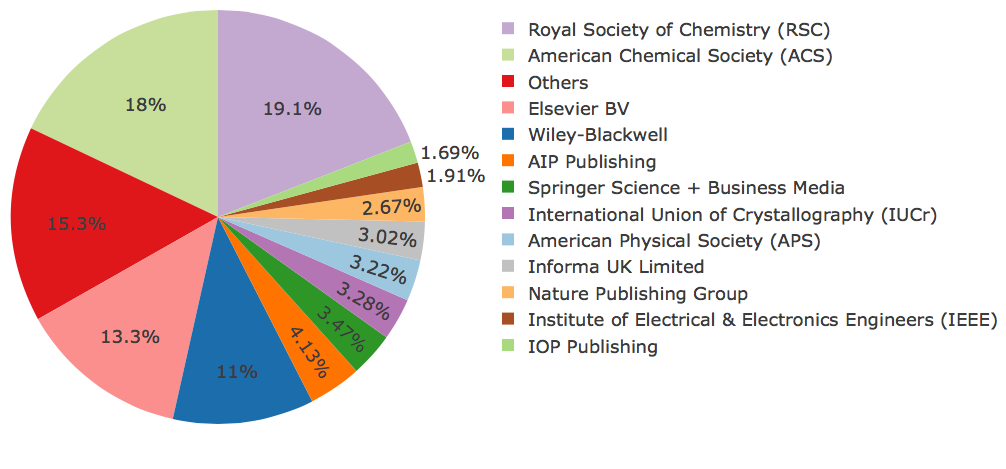
\includegraphics[scale=0.4]{Data_Acquisition/uk_publishers_pie.png}
    \caption{Articles grouped by publisher in the UK Doi database published by by each publisher. Only the top 12 publishers are shown.}
     \label{fig:UKPUBPI}
\end{figure}

The corpus of combined titles and abstracts of the complete training database was then examined. The word frequencies across all the data were found to be approximately Zipfian, with a gradient of-1.11\footnote{A Zipfian distribution is a subset of the Pareto distribution, stating that the frequency of a word is $\propto$ to its ranking in the word frequencies table. Ideally, the gradient of a log(frequency) vs log(rank) should be -1.0 \cite{zipf}} See figure \ref{fig:ZIPF}
\begin{figure}[H]
    \centering
    \textbf{Approximate Ziphian Distribution}\par\medskip
    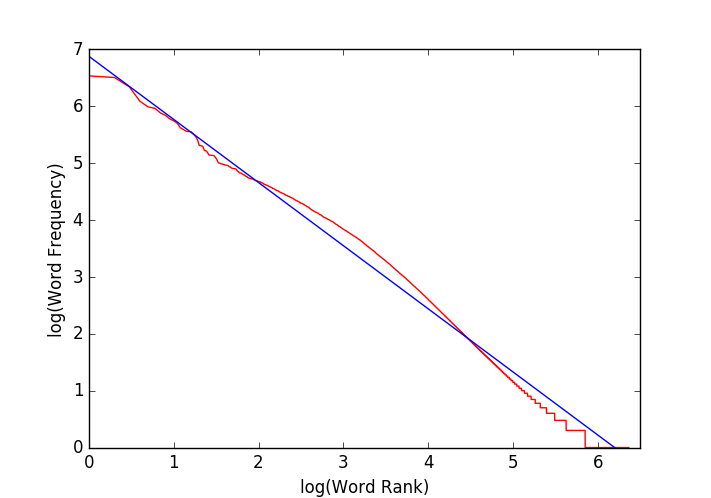
\includegraphics[scale=0.4]{Data_Acquisition/zipf.png}
    \caption{The log Frequency of words vs the log of their position in the rank in the word frequency table in blue. Best fit line in Red, gradient = -1.11, intercept 6.3. }
     \label{fig:ZIPF}
\end{figure}
A summary of the corpus statistics are shown below:
\begin{table}[h!]
\label{tab:CORPUS STATS}
\caption{Titles and Abstracts in Training Database}
\begin{center}
\begin{tabular}{||l|c||}
\hline
Total Word Count & 61,296,410\\
Total Unique Words & 2,326,725\\
Total Sentence Count & 464,712\\
Mode Words per Title &  11\\
Mean Words per Title &  12.2\\
Mode Words per Abstract & 156\\
Mean Words per Abstract & 119.7\\
Mode Sentences per Abstract & 4\\
Mean Sentences per Abstract & 5.4\\
\hline
\end{tabular}
\end{center}
\end{table}

\label{sec:SCRAPEANALYSIS}
